\documentclass[titlepage]{jsarticle}
\usepackage{amsmath,amssymb}
\usepackage{enumerate}
\usepackage[dvipdfmx]{graphicx}
\usepackage[dvipdfmx]{color}
\usepackage{here}
\usepackage{breqn}
\usepackage{amsthm}
\theoremstyle{definition}
\usepackage{bm}
\newtheorem{Ex}{問題}
%\newtheorem*{Ex*}{演習問題}
\newtheoremstyle{mystyle}%   % スタイル名
    {}%                      % 上部スペース
    {}%                      % 下部スペース
    {\normalfont}%           % 本文フォント
    {}%                      % インデント量
    {\bf}%                   % 見出しフォント
    {}%                      % 見出し後の句読点, '.'
    { }%                     % 見出し後のスペース, ' ' or \newline
    {\underline{\thmname{#1}\thmnumber{#2}\thmnote{(#3)}}}%
                             % 見出しの書式 (can be left empty, meaning `normal')
\theoremstyle{mystyle} % スタイルの適用
\newtheorem*{Def}{Def}
\newtheorem*{theo}{Theorem}
\newtheorem*{lem}{Lemma}
\newtheorem{ex}{example}
\newtheorem*{col}{Corollary}
\renewcommand{\footnotesize}{\normalsize}
\usepackage{latexsym}
\usepackage{color}
\usepackage{listings,jvlisting}
\def\qed{\hfill$\Box$}
\lstset{
language={Python},
backgroundcolor={\color[gray]{.85}},
basicstyle={\footnotesize},
identifierstyle={\footnotesize},
commentstyle={\footnotesize\ttfamily \color[rgb]{0,0.5,0}},
keywordstyle={\footnotesize\bfseries \color[rgb]{1,0,0}},
ndkeywordstyle={\footnotesize},
stringstyle={\footnotesize\ttfamily \color[rgb]{0,0,1}},
frame={tb},
breaklines=true,
columns=[l]{fullflexible},
numbers=left,
xrightmargin=0zw,
xleftmargin=3zw,
numberstyle={\scriptsize},
stepnumber=1,
numbersep=1zw,
morecomment=[l]{//}
}
\title{スパース推定100問 with python 解答}
\author{青嶋研究室\\
石川美果\\
海野哲也\\
中田健斗\\}
\date{\today}
\begin{document}
\large
\maketitle
\newpage
\tableofcontents


\newpage
\section{第1章解答}
\begin{Ex}
展開すると

\begin{equation}
\begin{split}
\label{ichi}
\begin{bmatrix}
\displaystyle\frac{\partial}{\partial \beta_1}\sum_{i=1}^N\left(y_i-\sum_{k=1}^p\beta_kx_{i,k}\right)^2\\
\vdots\\
\displaystyle\frac{\partial}{\partial \beta_p}\sum_{i=1}^N\left(y_i-\sum_{k=1}^p\beta_kx_{i,k}\right)^2
\end{bmatrix}&=-2\begin{bmatrix}
\displaystyle\sum_{i=1}^N x_{i,1}\left(y_i-\sum_{k=1}^p x_{i,k}\beta_k\right)\\
\vdots\\
\displaystyle\sum_{i=1}^N x_{i,p}\left(y_i-\sum_{k=1}^p x_{i,k}\beta_k\right)
\end{bmatrix}\\
&=-2\begin{bmatrix}
x_{1,1}& \cdots & x_{N,1}\\
\vdots & \ddots & \vdots\\
x_{N,1} & \cdots & x_{N,p}
\end{bmatrix}\begin{bmatrix}
y_1-\sum_{k=1}^p x_{1,k}\beta_k\\
\vdots\\
y_N-\sum_{k=1}^p x_{N,k}\beta_k
\end{bmatrix}\\
&=-2X^T(y-X\beta)
\end{split}
\end{equation}
となることから等式が成立する.さらに$X^T X$が正則ならば,$\|y-X\beta\|_2^2$を最小にする$\beta$は
$$\begin{bmatrix}
\frac{\partial}{\partial \beta_1}\|y-X\hat{\beta}\|^2\\
\vdots\\
\frac{\partial}{\partial \beta_p}\|y-X\hat{\beta}\|^2
\end{bmatrix} = {\bm 0}$$
を満たすので,(\ref{ichi})式より
\begin{align*}
-2X^t(y-X\hat{\beta}) &= 0\\
X^T X\hat{\beta} &= X^Ty\\
\therefore \hat{\beta} = (X^T X)^{-1}X^T y
\end{align*}
となることがわかる.さらに,求める関数linerをpythonで構成する際のソースコードは以下の通り.
\begin{lstlisting}[basicstyle = \ttfamily\footnotesize, frame = single]
def linear(X,y):
    p = X.shape[1]
    x_bar = np.zeros(p)
    for j in range(p):
        x_bar[j] = np.mean(X[:,j])
    for j in range(p):
        X[:,j] = X[:, j] - x_bar[j]
    y_bar=np.mean(y)
    y = y - y_bar
    "beta" "=" "np.dot("
        "np.linalg.inv(np.dot(X.T,X)),np.dot(X.T,y)"
    ")" #空欄(1) 
     "beta_0 = y_bar - np.dot(x_bar,beta)"#空欄(2)
    return beta, beta_0
\end{lstlisting}\qed\\
\end{Ex}
%%%%%%%%%%%%%%%%%%%%%%1
\begin{Ex}
\noindent(a) $f(x)=x$

まず、関数$f$が凸であることを示す。
任意の$0<\alpha<1$ と $x,y\in\mathbb{R}$について、
\begin{equation*}
\{\alpha f(x) + (1 - \alpha) f(y)\} - f(\alpha x + (1 - \alpha) y)= \alpha x + (1 - \alpha) y - \alpha x - (1 - \alpha) y=0\geq 0
\end{equation*}
\noindent となる。よって、$f(\alpha x - (1 - \alpha) y)\leq\alpha f(x) + (1 - \alpha) f(y)$が成り立つので、関数$f$は 凸である。

次に、$x_0 = 0$ における $\partial f(x_0)$を求める。凸関数$f$は、$x_0=0$で微分可能なので、$\partial f(x_0)$は$f^{\prime}(x_0)=1$のみとなる。よって、$\partial f(x_0)=\{1\}$となる。
\vskip\baselineskip
\noindent(b) $f(x)=|x|$

まず、関数$f$が凸であることを示す。
任意の$0<\alpha<1$ と $x,y\in\mathbb{R}$について、

\begin{equation*}
f(\alpha x + (1 - \alpha) y) \leq \alpha f(x) + (1 - \alpha) f(y)
\end{equation*}

\noindent が成り立つことを示せばよい。
\begin{equation*}
\alpha f(x) + (1 - \alpha) f(y)=\alpha |x| + (1 - \alpha)|y|, f(\alpha x + (1 - \alpha) y)
=|\alpha x + (1 - \alpha) y|
\end{equation*}

\noindent となり、両辺非負であるため、右辺の二乗から左辺の二乗を引くと、
\begin{equation*}
(\alpha |x| + (1 - \alpha)|y|)^2 - (|\alpha x + (1 - \alpha) y|)^2=2\alpha (1 - \alpha)(|xy| - xy) \geq 0
\end{equation*}

\noindent となる。よって、$f(\alpha x - (1 - \alpha) y)\leq \alpha f(x) + (1 - \alpha) f(y)$が成り立つので、関数$f$は 凸である。

次に、$x_0 = 0$ における $\partial f(x_0)$を求める。任意の$x\in\mathbb{R}$について、$f(x) \geq f(x_0) + z(x-x_0)$ であるような$z \in\mathbb{R}$を求めればよい。

上の不等式は、$|x| \geq zx$と変形できる。よって、任意の$x\in\mathbb{R}$について、$|x| \geq zx$となるような$z \in\mathbb{R}$を求める。このとき、

\begin{equation*} 
任意のx\in\mathbb{R}で|x| \geq zx\Leftrightarrow|z| \leq 1
\end{equation*}

\noindent が成り立つ。実際、任意の$x\in\mathbb{R}$で$|x| \geq zx$であれば、$x>0$では$z \leq 1$が、$x<0$では$z \geq -1$が、$x=0$では$z$は任意の実数が成り立つことが必要である。よって、$|z| \leq 1$となる。逆に、$|z| \leq 1$であれば、$zx\leq |z||x|\leq |x|$が任意の$x$で成立する。以上より、上の同値性が成り立つ。よって、$\partial f(x_0)= [-1, 1]$となる。
\end{Ex}
%%%%%%%%%%%%%%%%%%%%%%%%%%%%%%%%%%%%%%%%%%2
\begin{Ex}

\end{Ex}
%%%%%%%%%%%%%%%%%%%%%%%%%%%%%%%%%%%%%%%%%%%%%3
\begin{Ex}\mbox{}\\
\begin{enumerate}[(a)]
\item 実数$x\in\mathbb{R}$を任意にとって固定する.$x=x_0$ならば等式
$$f(x)=f(x_0)+f'(x_0)(x-x_0)$$
が成立するので$x\neq x_0$とする.このとき,凸関数の定義より任意の$0<\alpha<1$に対して
\begin{align*}
f(\alpha x+(1-\alpha)x_0)\leq \alpha f(x)+(1-\alpha)f(x_0)
\end{align*}
が成立するので上式を変形して
\begin{align*}
f(\alpha x+(1-\alpha)x_0)-f(x_0)&\leq \alpha (f(x)-f(x_0))\\
f(x)-f(x_0)&\geq \frac{f(\alpha x+(1-\alpha)x_0)-f(x_0)}{\alpha}\\
\therefore f(x)&\geq f(x_0)+\frac{f(\alpha x+(1-\alpha)x_0)-f(x_0)}{\alpha(x-x_0)}(x-x_0)
\end{align*}
が得られる.$0<\alpha<1$は任意であったので,$\alpha\searrow 0$とすることで
\begin{align*}
f(x)\geq f(x_0)+f'(x_0)(x-x_0)
\end{align*}
となることがわかる.上式で実数$x$は任意にとれたので,求めたい不等式が示せた.\\

\item まず$\partial f(x_0)$は空集合でないことに注意する.実際(a)の結果より,
$$f(x)\geq f(x_0)+f'(x_0)(x-x_0)$$
が成立するので$f'(x_0)\in \partial f(x_0)$が成立している.\\

実数$z$が$z\in \partial f(x_0)$を満たしているとする.すなわち,任意の$x\in\mathbb{R}$に対して
\begin{equation}
\label{retsu}
f(x)\geq f(x_0)+z(x-x_0)
\end{equation}
が成立していたとする.このとき,上式を変形することで$x>x_0$の範囲において
\begin{align*}
z\leq \frac{f(x)-f(x_0)}{x-x_0}
\end{align*}
となることが要請されるので
\begin{align}
\label{migi}
z\leq \lim_{x\searrow x_0}\frac{f(x)-f(x_0)}{x-x_0}
\end{align}
となる必要がある.一方で,(\ref{retsu})式より$x<x_0$の範囲において
\begin{align*}
z\geq \frac{f(x)-f(x_0)}{x-x_0}
\end{align*}
となることが要請されるので
\begin{align}
\label{hidari}
z\geq \lim_{x\nearrow x_0}\frac{f(x)-f(x_0)}{x-x_0}
\end{align}
となる必要がある.以上(\ref{migi}),(\ref{hidari})式より
\begin{align*}
\lim_{x\nearrow x_0}\frac{f(x)-f(x_0)}{x-x_0}\leq z\leq \lim_{x\searrow x_0}\frac{f(x)-f(x_0)}{x-x_0}
\end{align*}
が成立するので,これと上式の最左辺と最右辺を見ることで
$$z\in \partial f(x_0)\Rightarrow z = f'(x_0)$$
が得られる.$f'(x_0)\in\partial f(x_0)$であったので,これより$\partial f(x_0)=\{f'(x_0)\}$が示せた.\qed\\
\end{enumerate}
\end{Ex}
%%%%%%%%%%%%%%%%%%%%%%%%%%%%%%%4
\begin{Ex}
以下では、$x<0, x=0, x>0$で場合分けして、$f(x)$の極小値を求める。$x\ne0$では通常の微分ができ、$f(x)=|x|$の$x=0$での劣微分が$[-1, 1]$であることに注意する。

\noindent(a) $f(x)=x^2-3x+|x|$

\begin{equation*}
f(x)=x^2-3x+|x|=
  \begin{cases}
  x^2-3x+x &  (x\geq0)\\
  x^2-3x-x &  (x<0)
  \end{cases}
=
  \begin{cases}
  x^2-2x &  (x\geq0)\\
  x^2-4x &  (x<0)
  \end{cases}
\end{equation*}

\begin{equation*}
f'(x)=(x^2-3x+|x|)'=
  \begin{cases}
  2x-2 &  (x<0)\\
  2x-3+[-1, 1] &  (x=0)\\
  2x-4 & (x>0)
  \end{cases}
=
  \begin{cases}
  2x-2 &  (x<0)\\
  -3+[-1, 1] &  (x=0)\\
  2x-4 & (x>0)
  \end{cases}
\end{equation*}

\begin{equation*}
  =
  \begin{cases}
  2x-2 &  (x<0)\\
  [-4, -2] &  (x=0)\\
  2x-4 & (x>0)
  \end{cases}
\end{equation*}

よって、$0\notin[-4, -2]$であるので、極小値は$x=1$のとき、$-1$となる。また、$-2\leq x \leq2$のグラフは、図1のようになる。

\noindent(b) $f(x)=x^2+x+2|x|$

\begin{equation*}
f(x)=x^2+x+2|x|=
  \begin{cases}
  x^2+x+2x &  (x\geq0)\\
  x^2+x-2x &  (x<0)
  \end{cases}
=
  \begin{cases}
  x^2+3x &  (x\geq0)\\
  x^2-x &  (x<0)
  \end{cases}
\end{equation*}

\begin{equation*}
\begin{split}
f'(x)=(x^2+x+2|x|)' & =
  \begin{cases}
  2x+3 &  (x<0)\\
  2x+1+2[-1, 1] &  (x=0)\\
  2x-1 & (x>0)
  \end{cases}
 \\
 & =
  \begin{cases}
  2x+3 &  (x<0)\\
  1+2[-1, 1] &  (x=0)\\
  2x-1 & (x>0)
  \end{cases}
\\
 & =
  \begin{cases}
  2x+3 &  (x<0)\\
  [-1, 3] &  (x=0)\\
  2x-1 & (x>0)
  \end{cases}
\end{split}
\end{equation*}

よって、$0\in[-1, 3]$であるので、極小値は$x=0$のとき、$0$となる。また、$-2\leq x \leq2$のグラフは、図2のようになる。

\begin{figure}[H]
  \begin{minipage}[]{0.52\linewidth}
    \centering
    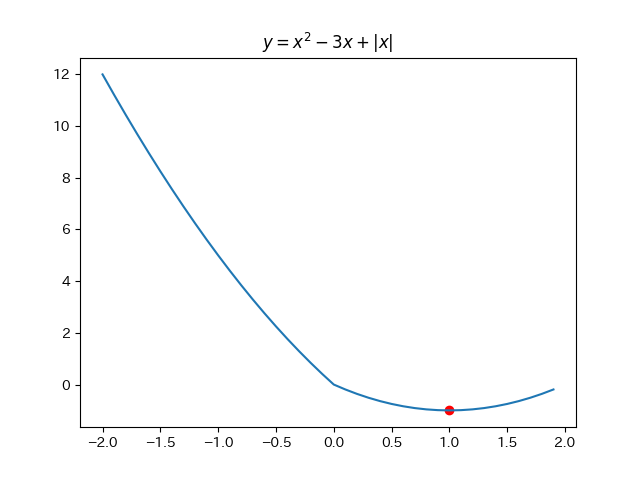
\includegraphics[keepaspectratio, scale=0.43]{mondai5(1).png}
    \caption{$f(x)=x^2-3x+|x|$}
  \end{minipage}
  \begin{minipage}[]{0.52\linewidth}
    \centering
    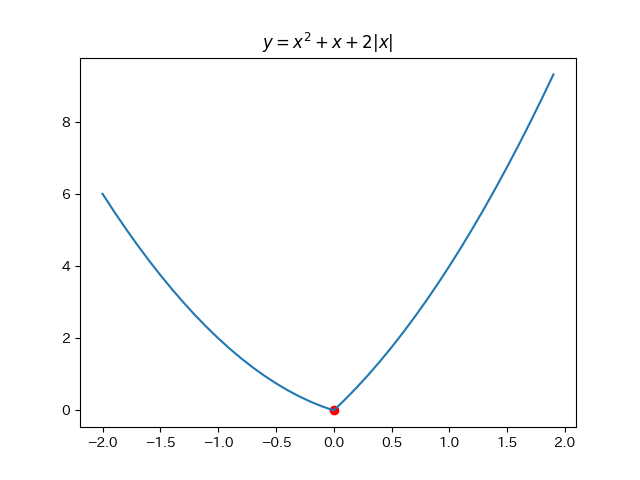
\includegraphics[keepaspectratio, scale=0.43]{mondai5(2).png}
    \caption{$f(x)=x^2+x+2|x|$}
  \end{minipage}
\end{figure}
\end{Ex}
%%%%%%%%%%%%%%%%%%%%%%%%%%%%%%%%%%%%%%%%5
\begin{Ex}

\end{Ex}
%%%%%%%%%%%%%%%%%%%%%%%%%%%%%%%%%%%%%%%6
\begin{Ex}\mbox{}\\
\begin{enumerate}[(a)]
\item 各$x\in \mathbb{R}$について場合分けして考える.\\
\begin{description}
\item[$x>\lambda$のとき]
この場合$x>0$かつ$|x|-\lambda\geq 0$であることより${\rm sign}(x)=1$かつ$(|x|-\lambda)_+=x-\lambda$が得られる.したがって
\begin{align*}
\mathcal{S}_{\lambda}(x)&=x-\lambda={\rm sign}(x)(|x|-\lambda)_+
\end{align*}
となることがわかる.\\

\item[$|x|\leq \lambda$のとき]
この場合$|x|-\lambda\leq 0$であることから$(|x|-\lambda)_+=0$となるので
\begin{align*}
\mathcal{S}_{\lambda}(x)={\rm sign}(x)(|x|-\lambda)_+=0
\end{align*}
が得られる.\\

\item[$x<-\lambda$のとき]
この場合$x<0$かつ$|x|-\lambda \geq 0$であることより${\rm sign}(x)=-1$かつ$(|x|-\lambda)_+=-x-\lambda$が得られる.したがって
\begin{align*}
\mathcal{S}_{\lambda}(x)&=x+\lambda=-(-x-\lambda)={\rm sign}(x)(|x|-\lambda)_+
\end{align*}
となることがわかる.\\
\end{description}
以上より任意の$x\in \mathbb{R}$に対して
$$\mathcal{S}_{\lambda}(x)={\rm sign}(x)(|x|-\lambda)_+$$
とかけることが示せた.\\

\item (a)で示した対応をPythonに実行させるコードは以下の通り.
\begin{lstlisting}[basicstyle = \ttfamily\footnotesize, frame = single]
def soft_th(lam,x):
    return np.sign(x) * np.maximum(np.abs(x) - lam,0)
\end{lstlisting}
さらに$\lambda=5$の場合の関数$\mathcal{S}_{\lambda}$のグラフを出力すると下のようになる
\subsection*{入力}
\begin{lstlisting}[basicstyle = \ttfamily\footnotesize, frame = single]
x = np.arange(-10,10,0.1)
y = soft_th(5,x)
plt.plot(x,y,c = "black")
plt.title(r"${\cal S}_\lambda(x)$",size = 24)
plt.plot([-5,-5],[-4,4],c = "blue",linestyle = "dashed")
plt.plot([5,5],[-4,4],c = "blue",linestyle = "dashed")
plt.text(-2,1,r"$\lambda = 5$",c ="red",size = 16)
\end{lstlisting}

\subsection*{出力結果}
\begin{figure}[H]
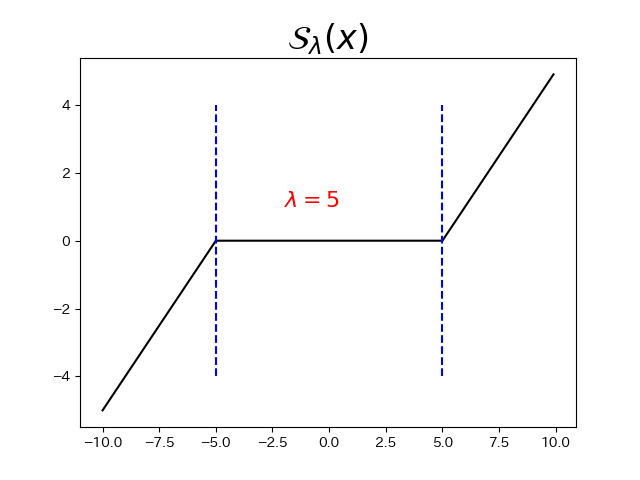
\includegraphics[width=10cm]{sl.png}
\end{figure}
確かに$\lambda=5$における関数$\mathcal{S}_{\lambda}$の動作と,定義したsoft\_thが一致していることが確認できる.\qed\\
\end{enumerate}
\end{Ex}
%%%%%%%%%%%%%%%%%%%%%%%%%%%%7
\begin{Ex}
まず、コードを以下に示す。
\begin{lstlisting}[basicstyle = \ttfamily\footnotesize, frame = single]
def linear_lasso(X, y, lam=0, beta=None):
    n, p = X.shape
    if beta is None:
        beta = np.zeros(p)
    X, y, X_bar, X_sd, y_bar = centralize(X, y)   # 中心化
    eps = 1
    beta_old = copy.copy(beta)
    while eps > 0.00001:    # このループの収束を待つ
        for j in range(p):
            r = (1) y
            for k in range(p):
                if j != k:
                    r = r - X[:, k] * beta[k]
            z = (np.dot(r, X[:, j]) / n) / (np.dot(X[:, j], X[:, j]) / n)
            beta[j] = soft_th(lam, z)
        eps = np.linalg.norm(beta - beta_old, 2)
        beta_old = copy.copy(beta)
    beta = beta / X_sd   # 各変数の係数を正規化前のものに戻す
    beta_0 = (2) y_bar - np.dot(X_bar, beta)
    return beta, beta_0
\end{lstlisting}

実行結果は以下のようになる。
\begin{figure}[H]
\centering
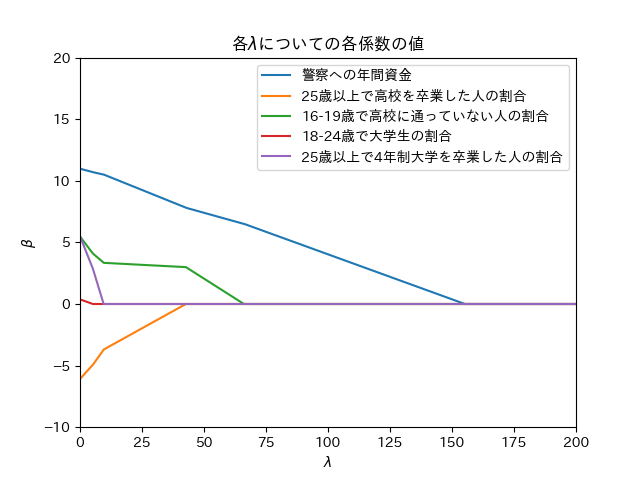
\includegraphics[scale=0.7] {Lasso1.png}
\end{figure}

次に、$\lambda=10,50,100$で、係数が0の変数のうち、何個がどのように変わるか調べる。


$\lambda=10$のとき、Lassoの実行結果は、(10.47248183, -3.64521939,  3.33650908,  0, 0)となり、非ゼロ係数が3個、ゼロ係数が2個という結果となった。$\lambda=50$のとき、Lassoの実行結果は、(7.40608466, 0,  2.0596716 , 0, 0)となり、非ゼロ係数が2個、ゼロ係数が3個という結果となった。$\lambda=100$のとき、Lassoの実行結果は、( 4.03117071, 0, 0, 0, 0)となり、非ゼロ係数が1個、ゼロ係数が4個という結果となった。
\end{Ex}
%%%%%%%%%%%%%%%%%%%%%%8
\begin{Ex}

\end{Ex}
%%%%%%%%%%%%%%%%%%%%%%%%%%%9
\begin{Ex}
空欄を埋めたプログラムは以下の通り
\begin{lstlisting}[basicstyle = \ttfamily\footnotesize, frame = single]
def warm_start(X, y, lambda_max=100):
    dec = np.round(lambda_max / 50)
    lambda_seq = np.arange(lambda_max, 1, -dec)
    r = len(lambda_seq)
    p = X.shape[1]
    beta = np.zeros(p)
    coef_seq = np.zeros((r, p))
    for k in range(r):
        beta, _ = linear_lasso(X, y, lambda_seq[k], beta)
        coef_seq[k, :] = beta
    return coef_seq
\end{lstlisting}
\begin{lstlisting}[basicstyle = \ttfamily\footnotesize, frame = single]
df = np.loadtxt("crime.txt", delimiter="\t")
X = df[:, [i for i in range(2, 7)]]
p = X.shape[1]
y = df[:, 0]
coef_seq = warm_start(X, y, 200)
lambda_max = 200
dec = round(lambda_max / 50)
lambda_seq = np.arange(lambda_max, 1, -dec)
plt.ylim(np.min(coef_seq), np.max(coef_seq))
plt.xlabel(r"$\lambda$")
plt.ylabel("係数")
plt.xlim(0, 200)
plt.ylim(-10, 20)
for j in range(p):
    plt.plot(lambda_seq, coef_seq[:, j])
\end{lstlisting}
出力結果は下の通り
\begin{figure}[H]
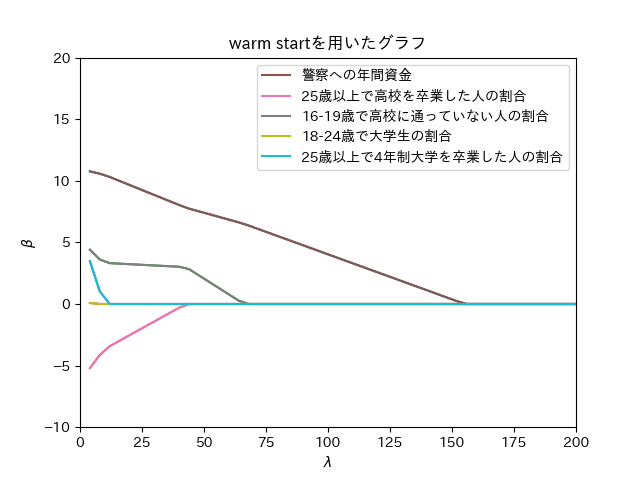
\includegraphics[width=10cm]{crime.png}
\end{figure}
また$\lambda$の値が$\displaystyle {\rm max}_{1\leq j\leq p}\left|\frac{1}{N}\sum_{i=1}^Nx_{i,j}y_i\right|$よりも大きいとき,全ての$j=1,\cdots,p$に対して
$$\beta_j =0\;{\rm かつ}\; r_{i,j}=y_i$$
が成立していることから




\end{Ex}
%%%%%%%%%%%%%%%%%%%%%%%%%%%%%%%10
\begin{Ex}
まず、$X^TX$の固有値が$\gamma_1, ... , \gamma_p$のとき、逆行列が存在しない条件を$\gamma_1, ... , \gamma_p$を用いて表す。$X^TX$の行列式$det(X^TX)$が固有値の積に等しい、つまり、$det(X^TX)=\gamma_1\cdots\gamma_p$であることを考えると、
\begin{equation*}
\begin{split}
X^TXの逆行列が存在しない \Leftrightarrow det(X^TX)=0 &\Leftrightarrow \gamma_1\cdots\gamma_p=0 \\
&\Leftrightarrow  \gamma_i=0となるようなi\in\{1, ... , p\}が存在する
\end{split}
\end{equation*}

\noindent となる。よって、求める条件は、$\gamma_i=0$となるような$i\in\{1, ... , p\}$が存在するとなる。

次に、$X^TX+N\lambda I$の固有値が$\gamma_1+N\lambda, ... , \gamma_p+N\lambda$となることを示す。$X^TX+N\lambda I$の固有値$t$は、

\begin{equation*}
det(X^TX+N\lambda I-tI)=0 \Rightarrow det(X^TX-(t-N\lambda)I)=0 
\end{equation*}
であり、$X^TX$の固有値が$\gamma_1, ... , \gamma_p$であることを考えると、

\begin{equation*}
t-N\lambda=\gamma_1, ... , t-N\lambda=\gamma_p \Rightarrow t=\gamma_1+N\lambda, ... , t=\gamma_p+N\lambda
\end{equation*}
となる。よって、題意が示された。

最後に、$\lambda>0$である限り、$X^TX+N\lambda I$には逆行列が必ず存在することを示す。$X^TX$は非負定値であるので、固有値$\gamma_1, ... , \gamma_p$はすべて非負である。よって、$\lambda>0, N>0$であるので、$X^TX+N\lambda I$の固有値$\gamma_1+N\lambda, ... , \gamma_p+N\lambda$はすべて正となる。以上より、その積である$X^TX+N\lambda I$の行列式は正となるので、$X^TX+N\lambda I$は正則である。つまり、逆行列が必ず存在する。
\end{Ex}
%%%%%%%%%%%%%%%%%%%%%%%%%%%11
\begin{Ex}

\end{Ex}
%%%%%%%%%%%%%%%%%%%%%%%%%%%%12
\begin{Ex}
関数ridgeは以下のようにして構成できる
\begin{lstlisting}[basicstyle = \ttfamily\footnotesize, frame = single]
def ridge(X, y, lam=0):
    n, p = X.shape
    X, y, X_bar, X_sd, y_bar = centralize(X, y)
    beta = np.dot(
        np.linalg.inv(np.dot(X.T, X) + n * lam * np.eye(p)),
        np.dot(X.T, y)
    )
    beta = beta / X_sd
    beta_0 = y_bar - np.dot(X_bar, beta)
    return beta, beta_0
\end{lstlisting}
実行結果を確認する
\begin{lstlisting}[basicstyle = \ttfamily\footnotesize, frame = single]
df = np.loadtxt("crime.txt", delimiter="\t")
X = df[:, [i for i in range(2, 7)]]
y = df[:, 0]
linear(X, y)
\end{lstlisting}
\begin{lstlisting}[basicstyle = \ttfamily\footnotesize, frame = single]
(array([10.98067026, -6.08852939,  5.4803042 ,  0.37704431,  5.50047122]), 489.64859696903386)
\end{lstlisting}
\begin{lstlisting}[basicstyle = \ttfamily\footnotesize, frame = single]
ridge(X,y)
\end{lstlisting}
\begin{lstlisting}[basicstyle = \ttfamily\footnotesize, frame = single]
(array([10.98067026, -6.08852939,  5.4803042 ,  0.37704431,  5.50047122]), 717.96)
\end{lstlisting}
\begin{lstlisting}[basicstyle = \ttfamily\footnotesize, frame = single]
ridge(X,y)
\end{lstlisting}
\begin{lstlisting}[basicstyle = \ttfamily\footnotesize, frame = single]
(array([ 0.0563518 , -0.01976397,  0.07786309, -0.0171218 , -0.0070393 ]), 717.96)
\end{lstlisting}
実行結果が一致していることが確認できた.
\end{Ex}
%%%%%%%%%%%%%%%%%%%%%%%%%%%%%%%%%%%%%%%%%13
\begin{Ex}
変更後のプログラムは以下のようになる。なお、横軸に対数を取ってもグラフが正確に描けるよう適宜プログラムの修正を行っている。

\begin{lstlisting}[basicstyle = \ttfamily\footnotesize, frame = single]
df = np.loadtxt("crime.txt", delimiter="\t")
X = df[:, [i for i in range(2, 7)]]
p = X.shape[1]
y = df[:, 0]
lambda_seq = np.arange(0.1, 200, 0.1)
plt.xlabel(r"log$\lambda$")
plt.ylabel(r"$\beta$")
plt.title(r"各log$\lambda$についての各係数の値")
labels = ["警察への年間資金", "25歳以上で高校を卒業した人の割合",
          "16-19歳で高校に通っていない人の割合",
          "18-24歳で大学生の割合", "25歳以上で4年制大学を卒業した人の割合"]
r = len(lambda_seq)
beta = np.zeros(p)
coef_seq = np.zeros((r, p))
for i in range(r):
    beta, beta_0 = ridge(X, y, lambda_seq[i])
    coef_seq[i, :] = beta
for j in range(p):
    plt.plot(np.log(lambda_seq), coef_seq[:, j], label=labels[j])
plt.legend(loc="upper right")
\end{lstlisting}

よって、これを実行し、グラフを表示させると以下のようになる。

\begin{figure}[H]
\centering
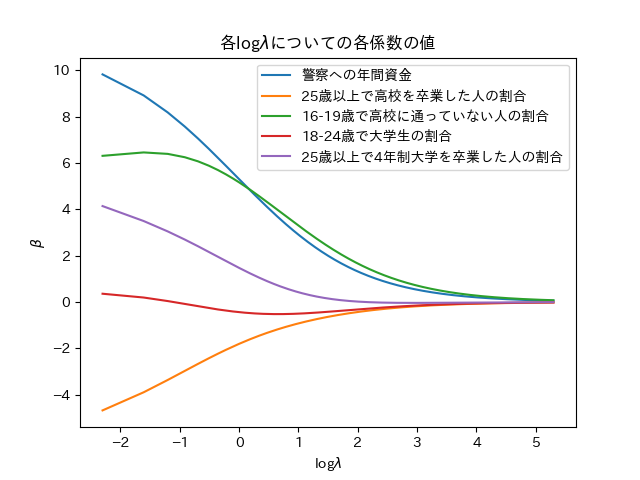
\includegraphics[scale=0.7] {monndai14.png}
\end{figure}
\end{Ex}
%%%%%%%%%%%%%%%%%%%%%%%%%%%%%%%14
\begin{Ex}

\end{Ex}
%%%%%%%%%%%%%%%%%%%%%%%%%%%%%%%15
\begin{Ex}
相異なる$k,l$について,$X$の第$k$列,第$l$列の$N$個の成分がすべて等しいする.\\
Ridgeにおける損失関数$L$は
$$L=\frac{1}{N}\sum_{i=1}^N(y_i-\beta_0-\sum_{j=1}^px_{i,j}\beta_j)+\lambda\sum_{j=1}^p \beta_j^2$$
となるので,$\beta_j,\beta_k$で$L$を偏微分すると
\begin{align*}
\frac{\partial L}{\partial \beta_k}&=-\frac{1}{N}\sum_{i=1}^Nx_{i,k}(y_i-\beta_0-\sum_{j=1}^px_{i,j}\beta_j)+\lambda \beta_k\\
\frac{\partial L}{\partial \beta_l}&=-\frac{1}{N}\sum_{i=1}^Nx_{i,l}(y_i-\beta_0-\sum_{j=1}^px_{i,j}\beta_j)+\lambda \beta_l
\end{align*}
となることがわかる.推定される$\beta_k,\beta_l$はこの偏微分の値が$0$になることから
\begin{align*}
\beta_k&=\frac{1}{\lambda N}\sum_{i=1}^Nx_{i,k}(y_i-\beta_0-\sum_{j=1}^px_{i,j}\beta_j)\\
\beta_l&=\frac{1}{\lambda N}\sum_{i=1}^Nx_{i,l}(y_i-\beta_0-\sum_{j=1}^px_{i,j}\beta_j)
\end{align*}
を満たしており,仮定より$x_{i,k}=x_{i,l}(i=1,\cdots,N)$であることから
\begin{align*}
\beta_k&=\frac{1}{\lambda N}\sum_{i=1}^Nx_{i,k}(y_i-\beta_0-\sum_{j=1}^px_{i,j}\beta_j)\\
&=\frac{1}{\lambda N}\sum_{i=1}^Nx_{i,l}(y_i-\beta_0-\sum_{j=1}^px_{i,j}\beta_j)=\beta_l
\end{align*}
となる.よって推定される$\beta_k,\beta_l$が等しくなることがわかる.\qed\\
\end{Ex}
%%%%%%%%%%%%%%%%%%%%%%%%%%%%%%%%16
\begin{Ex}
まず、コードを以下に示す。
\begin{lstlisting}[basicstyle = \ttfamily\footnotesize, frame = single]
n = 500
x = np.zeros((n, 6))
z = np.zeros((n, 5))
for k in range(2):
    z[:, k] = np.random.randn(n)
y = (1)3 * z[:, 0] - 1.5 * z[:, 1] + 2 * np.random.randn(n)
for j in range(3):
    x[:, j] = z[:, 0] + np.random.randn(n) / 5
for j in range(3, 6):
    x[:, j] = z[:, 1] + np.random.randn(n) / 5
lambda_seq = np.arange(0.1, 20, 0.1)
p = 6
r = len(lambda_seq)
coef_seq = np.zeros((r, p))
cols = ["blue", "red", "green", "yellow", "purple", "orange"]
for i in range(r):
    coef_seq[i, :], _ = (2)linear_lasso(x, y, lambda_seq[i])
for j in range(p):
    plt.plot(-np.log(lambda_seq), coef_seq[:, j] + 0.01 * j,
             c=cols[j], label="X"+str(j+1))
plt.xlabel(r"$-\log \lambda$")
plt.ylabel(r"$\beta$")
plt.legend(loc="upper left")
plt.title("Lasso")
\end{lstlisting}

実行結果は以下のようになる。

\begin{figure}[H]
\centering
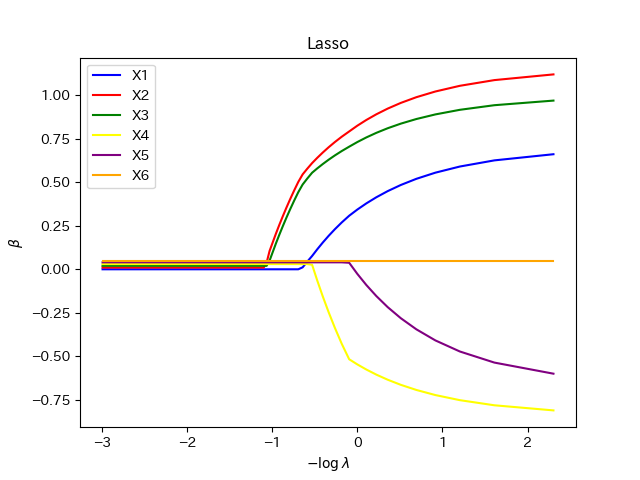
\includegraphics[scale=0.6] {monndai17.png}
\end{figure}
\end{Ex}
%%%%%%%%%%%%%%%%%%%%%%%%%%%%%%%%%%%%%%17
\begin{Ex}

\end{Ex}
%%%%%%%%%%%%%%%%%%%%%%%%%%%%%%%%%%%%%%%%18
\begin{Ex}
elasticネットは,例えば以下のようにして構成できる
\begin{lstlisting}[basicstyle = \ttfamily\footnotesize, frame = single]
def elastic_net(X, y, lam=0, alpha=1, beta=None):                     #
    n, p = X.shape
    if beta is None:
        beta = np.zeros(p)
    X, y, X_bar, X_sd, y_bar = centralize(X, y)   # 中心化
    eps = 1
    beta_old = copy.copy(beta)
    while eps > 0.00001:    # このループの収束を待つ
        for j in range(p):
            r = y
            for k in range(p):
                if j != k:
                    r = r - X[:, k] * beta[k]
            z = (np.dot(r, X[:, j]) / n)                                    ##
            beta[j] = (soft_th(lam * alpha, z)                              ##
                       / (np.dot(X[:, j], X[:, j]) / n + (1-alpha) * lam))  ##
        eps = np.linalg.norm(beta - beta_old, 2)
        beta_old = copy.copy(beta)
    beta = beta / X_sd   # 各変数の係数を正規化前のものに戻す
    beta_0 = y_bar - np.dot(X_bar, beta)
    return beta, beta_0
\end{lstlisting}
\end{Ex}

%%%%%%%%%%%%%%%%%%%%%%%%%%19
\begin{Ex}
linear\_lassoのパラメータ$\lambda$の最適な値を求める関数cv\_linear\_lassoは以下のようになる。

\begin{lstlisting}[basicstyle = \ttfamily\footnotesize, frame = single]
def cv_linear_lasso(x, y, alpha=1, k=10):
    lam_max = np.max(np.dot(x.T, y) / np.dot(x.T, x))
    lam_seq = np.array(range(100))**3 / 1000000 * lam_max
    n = len(y)
    m = int(n / k)
    r = n % k
    S_min = np.inf
    for lam in lam_seq:
        S = 0
        for i in range(k):
            if i < k - r:
                index = list(range(i*m, i*m + m))
            else:
                index = list(range(i*m + (i-k+r), i*m + (m+i-k+r+1)))
                # nをkで割れない場合
            _index = list(set(range(n)) - set(index))
            beta, beta0 = elastic_net(x[_index, ], y[_index], lam, alpha)
            z = np.linalg.norm((y[index] - beta0 - np.dot(x[index], beta)), 2)
            S = S + z**2
        if S < S_min:
            S_min = S.copy()
            lam_best = lam.copy()
            beta0_best = beta0.copy()
            beta_best = beta.copy()
    return lam_best, beta0_best, beta_best, S_min
\end{lstlisting}
\end{Ex}
%%%%%%%%%%%%%%%%%%%%%%%%%%%%%%%%%%%%%%%%%%%%%%%%%%%%20
\section{第2章解答}
\begin{Ex}

\end{Ex}
%%%%%%%%%%%%%%%%%%%%%%%%%%%%%%%%%%%%%%%%%%%%%%%%%%%%%21
\begin{Ex}
\begin{enumerate}[(a)]
\item 目的関数
$$L(\beta_0,\beta):=\sum_{i=1}^N \log\{1+\exp(-y_i(\beta_0+x_i^T \beta))\}$$
を$\beta_j(j=0,\cdots,p)$で偏微分するとき,$x_{i,0}=1(i=1,\cdots ,N),v_i :=\exp(-y_i(\beta_0+x_i^T \beta)) $と置くことで
\begin{align*}
\frac{\partial L}{\partial \beta_j}&=\sum_{i=1}^N\frac{-y_i\cdot x_{i,j}\exp(-y_i(\beta_0+x_i^T \beta))}{1+\exp(-y_i(\beta_0+x_i^T \beta))}\\
&=-\sum_{i=1}^N\frac{y_ix_{i,j} v_i}{1+v_i}
\end{align*}
とかけることより
\begin{align*}
\nabla L&=-\begin{pmatrix}
1 & \cdots & 1\\
x_{1,1} & \cdots & x_{N,1}\\
\vdots & \ddots & \vdots \\
x_{1,p} & \cdots & x_{N,p}
\end{pmatrix}\left(\begin{array}{c}
\frac{y_1 v_i}{1+v_1}\\
\vdots \\
\frac{y_1 v_N}{1+v_N}
\end{array}\right)=-X^T u
\end{align*}
と書くことができる.\\

\item (a)で求めた$\frac{\partial L}{\partial \beta_j}$をさらに$\beta_k$で偏微分すると
\begin{align*}
\frac{\partial^2 L}{\partial \beta_j \partial \beta_k}&=-\sum_{i=1}^N \left\{\frac{\partial v_i}{\partial \beta_k}\frac{\partial }{\partial v_i}\left(\frac{y_ix_{i,j}v_i}{1+v_i}\right)\right\}\\
&=\sum_{i=1}^Ny_i^2x_{i,j}x_{i,k}\frac{v_i}{(1+v_i)^2}\\
&=\sum_{i=1}^Nx_{i,j}x_{i,k}\frac{v_i}{(1+v_i)^2}\quad(\because y_i\in \{\pm 1\})
\end{align*}
となることより,
\begin{align*}
\nabla^2 L &=X^T\begin{pmatrix}
\frac{v_1}{(1+v_1)^2} & \cdots & 0\\
\vdots & \ddots & \vdots \\
0 & \cdots & \frac{v_N}{(1+v_N)^2}
\end{pmatrix}X\\
&=X^TWX
\end{align*}
と書くことができる.\\
\end{enumerate}
さらに,上記で求めた行列を用いて作成した,Newton法により値を更新していくプログラムの実行結果は下の通り.最上段が初期値($p+1$次元)を,最下段が推定された係数と実際の係数の$l2$ノルムを表す

\begin{lstlisting}[basicstyle = \ttfamily\footnotesize, frame = single]
#p=2
[ 0.63094861 -0.92697651 -0.91072333]
[ 0.86047835 -1.14017869 -1.35275858]
[ 0.95114002 -1.22561286 -1.50788179]
[ 0.96108609 -1.235      -1.52382468]
0.7609464718257709

#p=3
[-0.39248015 -0.60068543 -0.6049099  -1.33818295]
[-0.46124804 -0.72404346 -0.72430081 -1.87481017]
[-0.48976562 -0.77927907 -0.771821   -2.06096778]
[-0.49271985 -0.78517205 -0.77653638 -2.0784206 ]
0.7252842383848371

#p=4
[ 0.08141478 -0.68484112  0.70987333 -1.50021169  0.0729047 ]
[ 0.0575044  -0.92584186  1.0212524  -2.04351767  0.1381232 ]
[ 0.05396007 -1.0284011   1.15461278 -2.28043797  0.16276137]
[ 0.05397496 -1.04263046  1.17324641 -2.31351461  0.16560318]
[ 0.05398124 -1.04286421  1.17355273 -2.31405542  0.16564041]
1.183505858275822

#p=5
[-0.44735853  0.1753804   0.74519156 -0.75696786  0.95888674  0.52116991]
[-0.51760096 -0.84462375  0.78877956 -1.1092826   0.70638379 -0.42738666]
[-0.74273836 -0.84191146  1.08434294 -1.39660604  1.10210054 -0.30626662]
[-0.81581402 -0.91371154  1.18648688 -1.52188011  1.2140128  -0.32811659]
[-0.82315975 -0.9212835   1.19631503 -1.53466277  1.22504241 -0.33062673]
0.8536261412241056

#p=6
[-0.30254961 -0.65441239 -0.7671653   0.89556886  0.82291769 -1.8986078
  1.09200474]
[-0.93939836 -0.85281913  0.71360078  0.24822987  0.12968842  0.23661314
  0.79192553]
[-0.78674208 -0.88892596  0.19398896  0.61617608  0.47178312 -0.73113428
  1.06501684]
[-0.98383111 -1.13192227  0.26832396  0.75029806  0.56505247 -0.8264384
  1.33542463]
[-1.03257514 -1.1857139   0.28516761  0.78091463  0.59207949 -0.84812315
  1.40043966]
[-1.03483699 -1.18803046  0.28591791  0.7822523   0.59338503 -0.8490672
  1.40340034]
1.0691750340249508
\end{lstlisting}
$p$を大きくしていくごとに,シミュレーションの計算が発散してしまう回数が増えていった.\qed\\
\end{Ex}
%%%%%%%%%%%%%%%%%%%%%%%%%%%%%%%%%%%%%%%%%%%%%22

\begin{Ex}
\noindent(a) $\nabla L = -X^T u$より、$ -X^T u=0$を解けばよい。両辺に左から$-X$をかけると、$ XX^T u=0$となり、$rankX=rank(XX^T)=N$より、$XX^T$は逆行列を持つので、$u=0$でないと$ XX^T u=0$は定常階に到達しない。さらに、有限の$(\beta, \beta_0)$の値では$u=0$にならないので、$(\beta, \beta_0)$は発散する。\\[1mm]

\noindent(b) $L=\frac{1}{N}\sum_{i=1}^{N}log(1+exp\{-y_i (\beta_0+x_i\beta)\})$より、$-y_i (\beta_0+x_i\beta)>0$であれば、$(\beta, \beta_0)$よりも、$(2\beta, 2\beta_0)$のほうが$L$を小さくする。よって、$(\beta, \beta_0)$は発散する。\\[1mm]
\end{Ex}
%%%%%%%%%%%%%%%%%23
\begin{Ex}

\end{Ex}
%%%%%%%%%%%%%%%%%24
\begin{Ex}
\begin{enumerate}[(a)]
\item $\gamma_0\in\mathbb{R},\gamma\in\mathbb{R}^p$を任意にとって固定し,(2.25)式の指数部全てから$\gamma_0+x^T\gamma$を引いた式を変形していくと
\begin{align*}
&\hspace{-3cm}\frac{\exp(\beta_{0,k}+x^T\beta^{(k)}-(\gamma_0+x^T\gamma))}{\sum_{l=1}^K\exp(\beta_{0,k}+x^T\beta^{(l)}-(\gamma_0+x^T\gamma))}\\
&=\frac{\exp(-(\gamma_0+x^T\gamma))\exp(\beta_{0,k}+x^T\beta^{(k)})}{\exp(-(\gamma_0+x^T\gamma))\sum_{l=1}^K\exp(\beta_{0,k}+x^T\beta^{(l)})}\\
&=\frac{\exp(\beta_{0,k}+x^T\beta^{(k)})}{\sum_{l=1}^K\exp(\beta_{0,k}+x^T\beta^{(l)})}=P(Y=k\mid x)\\
\therefore P(Y=k\mid x)&=\frac{\exp(\beta_{0,k}+x^T\beta^{(k)}-(\gamma_0+x^T\gamma))}{\sum_{l=1}^K\exp(\beta_{0,k}+x^T\beta^{(l)}-(\gamma_0+x^T\gamma))}
\end{align*}
となり,等号が得られることがわかる.\\

\item $\beta_{j,1},\cdots,\beta_{j,K}$の値が求まったとき$(j=1,\cdots,p)$,$\displaystyle \sum_{k=1}^K|\beta_{j,k}-\gamma_j|$の値を最小にする$\gamma_j\in\mathbb{R}$を求めればよい.またそのような$\gamma_j$ は$\beta_{j,1},\cdots,\beta_{j,K}$の中央値になると文中で述べられているので,$\beta_{j,1},\cdots,\beta_{j,K}$を求めた後にそれらすべてから中央値を引けばよいことがわかる.\\

\item $\displaystyle \sum_{k=1}^K\beta_{0,k}$となるように設定されていることから,最初に$\beta_{0,1},\cdots,\beta_{0,K}$の値を求めた後,それらすべてから$\bar{\beta}:=\displaystyle \frac{1}{K}\sum_{k=1}^K\beta_{0,k}$を引いていることがわかる.\qed\\
\end{enumerate}
\end{Ex}
%%%%%%%%%%%%%%%%%%%%%%%%%%%%%%%%%%%%%%%%25
\begin{Ex}
コードは以下のようになる。

\begin{lstlisting}[basicstyle = \ttfamily\footnotesize, frame = single]
from sklearn.datasets import load_iris
iris = load_iris()
X = np.array(iris["data"])
y = np.array(iris["target"], dtype="float64")
cvfit3 = cvglmnet(x=X.copy(), y=y.copy(),
                  ptype="deviance", family="multinomial")
lam_min = cvfit1["lambda_min"]
beta = cvglmnetCoef(cvfit)
print(lam_min)
print(beta)

fig3 = plt.figure()
cvglmnetPlot(cvfit3)
fig3.savefig("img3.png")

K = 3
p = 5
n = 150
gamma = np.zeros((K, p))
for k in range(K):
    for j in range(p):
        gamma[k, j] = np.sum(beta[k][j])
v = np.zeros(n)
for i in range(n):
    max_value = -np.inf
    for k in range(K):
        value = gamma[k, 0] + np.dot(gamma[k, range(1, p)], X[i, :])
        if value > max_value:
            v[i] = k
            max_value = value
table_count(3, y, v)
\end{lstlisting}

\end{Ex}
%%%%%%%%%%%%%%%%%%%%%%%%%%%%26
\begin{Ex}

\end{Ex}
%%%%%%%%%%%%%%%%%%%%%%%%%%%%%27
\begin{Ex}
\begin{enumerate}[(a)]
\item (2.26)式は観測値$(x_1,y_1),\cdots,(x_N,y_N)$から得られる尤度関数で
$$\prod_{i=1}^N\frac{\mu_i^{y_i}}{y_i!}e^{-\mu_i}\quad (\mu_i = e^{\beta_0+x_i^T \beta})$$
となっている.この尤度関数のマイナス対数をとると
\begin{align*}
-\log\left(\prod_{i=1}^N\frac{\mu_i^{y_i}}{y_i!}e^{-\mu_i}\right)&=\sum_{i=1}^N\{\log(y_i!)-y_i\log(\mu_i)+\mu_i\}\\
&=\sum_{i=1}^N\{\log(y_i!)-y_i(\beta_0+x_i^T\beta)+e^{\beta_0+x_i^T\beta}\}\\
&=L(\beta_0,\beta)+\sum_{i=1}^N \log(y_i!)
\end{align*}
となる.最下段の$\beta_0,\beta$に関する最小化は$\frac{1}{N}L(\beta_0,\beta)$の$\beta_0,\beta$に関する最小化と同値であり,この式に正則化項をつけると
$$\frac{1}{N}L(\beta_0,\beta)+\lambda\|\beta\|_1$$
となる.このようにして(2.27)式が導出される.\\

\item $L(\beta_0,\beta)=\sum_{i=1}^N\{y_i(\beta_0+x_i^T \beta)-e^{\beta_0+ x_i^T \beta}\}$を$\beta_j(j=0,\cdots,p)$で微分すると
\begin{align*}
\frac{\partial L}{\partial \beta_j} &=\sum_{i=1}^N \{-y_i x_{i,j}+x_{i,j}e^{\beta_0+ x_i^T \beta}\}\\
&=-\sum_{i=1}^N x_{i,j}(y_i-e^{\beta_0+ x_i^T \beta})
\end{align*}
となる.ただし$x_{i,0}=1(i=1,\cdots,N)$とした.よって
\begin{align*}
\nabla L&=-\begin{pmatrix}
1 & \cdots & 1\\
x_{1,1} & \cdots & x_{N,1}\\
\vdots & \ddots & \vdots \\
x_{1,p} & \cdots & x_{N,p}
\end{pmatrix}\left(\begin{array}{c}
y_1-e^{\beta_0+x_1^T \beta}\\
\vdots\\
y_N-e^{\beta_0+x_N^T \beta}
\end{array}\right)
\end{align*}
となるので,
$$u=\left(\begin{array}{c}
y_1-e^{\beta_0+x_1^T \beta}\\
\vdots\\
y_N-e^{\beta_0+x_N^T \beta}
\end{array}\right)$$
とすれば$\nabla L = -X^T u$とかくことができる.\\

\item (b)で得られた$\frac{\partial L}{\partial \beta_j}$をさらに$\beta_k$で偏微分すると
\begin{align*}
\frac{\partial }{\partial \beta_k}\left(\frac{\partial L}{\partial \beta_j}\right)&=-\sum_{i=1}^N x_{i,j}x_{i,k}e^{\beta_0+x_i^T \beta}
\end{align*}
となることより
\begin{align*}
\nabla^2 L &=X^T \begin{pmatrix}
e^{\beta_0+x_1^T \beta} & \cdots & 0\\
\vdots & \ddots & \vdots \\
0 & \cdots & e^{\beta_0+x_N^T \beta}
\end{pmatrix}X
\end{align*}
となるので,
$$W = \begin{pmatrix}
e^{\beta_0+x_1^T \beta} & \cdots & 0\\
\vdots & \ddots & \vdots \\
0 & \cdots & e^{\beta_0+x_N^T \beta}
\end{pmatrix}$$
とすれば$\nabla^2 L =X^TWX$と書くことができる.\qed\\
\end{enumerate}
また掲載されているプログラムの空欄を埋めてコード,およびそれを実行した結果は下のようになる
\begin{lstlisting}[basicstyle = \ttfamily\footnotesize, frame = single]
def poisson_lasso(X, y, lam):
    p = X.shape[1]   # pはすべて1の列を含んでいる
    beta = np.random.randn(p)
    gamma = np.random.randn(p)
    while np.sum((beta - gamma) ** 2) > 0.0001:
        beta = gamma
        s = np.dot(X, beta)
        w = np.exp(s) #空欄1
        u = y - w #空欄2
        z = s + u / w #空欄3
        gamma_0, gamma_1 = W_linear_lasso(X[:, range(1, p)],
                                          z, np.diag(w), lam)
        gamma = np.block([gamma_0, gamma_1]).copy()
        print(gamma)
    return gamma

N = 100    
p = 3
X = np.random.randn(N, p)
X = np.concatenate([np.ones(N).reshape(N, 1), X], axis=1)
beta = np.random.randn(p + 1)
s = np.dot(X, beta)
y = np.random.poisson(lam=np.exp(s))
print(beta)
\end{lstlisting}
\begin{lstlisting}[basicstyle = \ttfamily\footnotesize, frame = single]
[-0.47085992 -0.31067144  0.30882489 -0.00316935] #真のbの値
[ 0.7654697  0.        -0.        -0.       ]
[ 0.05384126 -0.          0.          0.        ]
[-0.35865758 -0.          0.          0.        ]
[-0.4711855 -0.         0.         0.       ]
[-0.47801239 -0.          0.          0.        ]#推定されたb
\end{lstlisting}
推定された$\beta$がスパースなものであることが確認できた.\qed\\

\end{Ex}
%%%%%%%%%%%%%%%%%%%%%%%%%28
\begin{Ex}
実行結果は以下のようになる。
\begin{figure}[H]
 \centering
 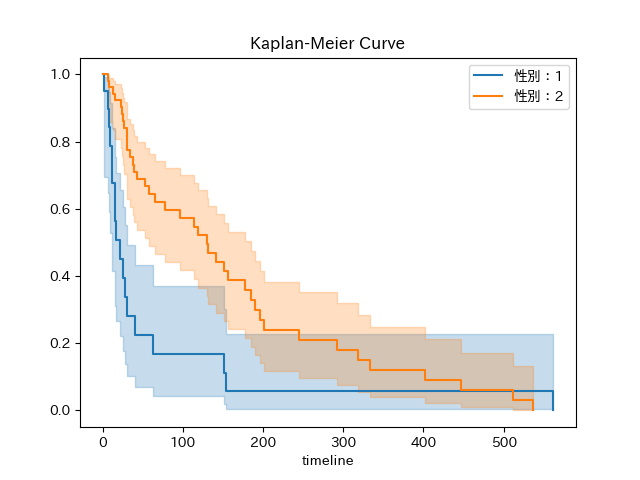
\includegraphics[keepaspectratio, scale=0.7]{seizonnkaiseki.png}
\end{figure}
\end{Ex}
%%%%%%%%%%%%%%%%%%%%%%%%%29
\begin{Ex}

\end{Ex}
%%%%%%%%%%%%%%%%%%%%%%%%%%30
\begin{Ex}
  \begin{enumerate}[(a)]

\item 関数$L$は
$$L(\beta) := -\sum_{i:\delta_i = 1}\log \frac{e^{x_i^T \beta}}{\sum_{j\in R_i}e^{x_j^T \beta}}$$
で定義されている.この関数$L$を$\beta_k$で偏微分すると

\begin{align*}
  \frac{\partial L}{\partial \beta_k}&=-\sum_{i:\delta_i = 1}\left\{x_{i,k}-\frac{\sum_{j\in R_i x_{j,k}\exp(x_j^T \beta)}}{\sum_{h\in R_i\exp(x_h^T \beta) }}\right\}\\
  &=-\sum_{i=1}^N x_{i,k}\left\{
    \delta_i - \sum_{j\in C_i}\frac{\exp(x_i^T \beta)}{\sum_{h\in R_j}\exp(x_h^T \beta)}
  \right\}
\end{align*}
とかくことができる.ここで,$S_i\alpha= \sum_{h\in R_i}\exp(x_h^T \beta)$としたときに
\begin{align*}
\sum_{i;\delta_i=1}\sum_{j\in R_j}\frac{x_{j,k}\exp(x_j^T \beta)}{S_i}&= \sum_{i=1}^N\sum_{i\in C_i}\frac{x_{j,k}\exp(x_j^T \beta)}{S_i}\\
&=\sum_{i=1}^N x_{i,k}\sum_{j\in C_i}\frac{\exp(x_i^T \beta)}{S_j}
\end{align*}
と変形できることより
\begin{align*}
  \frac{\partial L}{\partial \beta_k}&=
  -\sum_{i=1}^N x_{i,k}\left\{\delta_i - \sum_{j\in C_i}\frac{\exp(x_i^T \beta)}{\sum_{h\in R_j}\exp(x_h^T \beta)}\right\}
\end{align*}
となることがわかる.したがって
\begin{align*}
  \nabla L&=-X^T \left(\begin{array}{c}
    \delta_1- \sum_{j\in C_1}\frac{\exp(x_1^T \beta)}{\sum_{h\in R_j}\exp(x_h^T \beta)}\\
    \vdots \\
    \delta_N- \sum_{j\in C_N}\frac{\exp(x_1^T \beta)}{\sum_{h\in R_j}\exp(x_h^T \beta)}
  \end{array}\right)
\end{align*}
となることより,求める$u$は
$$u=\left(\begin{array}{c}
  \delta_1- \sum_{j\in C_1}\frac{\exp(x_1^T \beta)}{\sum_{h\in R_j}\exp(x_h^T \beta)}\\
  \vdots \\
  \delta_N- \sum_{j\in C_N}\frac{\exp(x_1^T \beta)}{\sum_{h\in R_j}\exp(x_h^T \beta)}
\end{array}\right)$$
とかける.\\

\item $\nabla^2 L$の各成分を変形していくと以下のようになる

\begin{align*}
  \frac{\partial L}{\partial \beta_k\partial\beta_l}&=
  \sum_{i=1}^N\sum_{j\in C_i}\frac{\partial}{\partial\beta_l}\left(\frac{\exp(x_i^T\beta)}{\sum_{h\in R_j}\exp(x_h^T\beta)}\right)\\
  &=\sum_{i=1}^Nx_{i,k}\sum_{j\in C_i}\frac{1}{(\sum_{r\in R_j}\exp(x_r^T\beta))^2}\left\{x_{i,l}\exp(x_i^T\beta)\sum_{s\in R_j}\exp(x_s^T\beta)\right.\\
  &\hspace{9cm}\left.-\exp(x_i^T\beta)\sum_{h\in R_j}x_{h,l}\exp(x_h^T \beta)\right\}\\
  &=\sum_{i=1}^N\sum_{h=1}^N x_{i,k}x_{h,l}\sum_{j\in C_i}\frac{\exp(x_i^T\beta)}{(\sum_{t\in R_j}\exp(x_t^T \beta))^2}\left\{I(i=h)\sum_{s\in R_j}\exp(x_s^T \beta)-I(h\in R_j)\exp(x_h^T \beta)\right\}
\end{align*}
とかける.ここで$W$の対角成分,すなわち$i=h$となる成分は
\begin{align*}
  w_{i} &=\sum_{j\in C_i}\frac{\exp(x_i^T\beta)}{(\sum_{t\in R_j}\exp(x_t^T \beta))^2}\left\{\sum_{s\in R_j}\exp(x_s^T \beta)-I(h\in R_j)\exp(x_i^T \beta)\right\}
\end{align*}
とかくことができ,
$$\delta_i =1,j\in R_i\Leftrightarrow i\in C_i$$
であることより$i=h$ならば$j\in C_i \Leftrightarrow i=h\in R_j$が得られる.したがって
$$\pi_{i,j}:=\frac{\exp(x_i^T \beta)}{\sum_{r\in R_j}\exp(x_i^T\beta)}$$
とすることで,$W$の各対角成分$w_i$は
\begin{align*}
  w_i&=
  \sum_{j\in C_i}\frac{\exp(x_i^T \beta)}{\sum_{r\in R_j}\exp(x_i^T\beta)}\left\{1-\frac{\exp(x_i-T \beta)}{\sum_{r\in R_j}\exp(x_i^T\beta)}\right\}=\sum_{j\in C_i}\pi_{i,j}(1-\pi_{i,j})
\end{align*}
とかける.\qed\\
\end{enumerate}


\end{Ex}
%%%%%%%%%%%%%%%%%%%%%%%%%%%%%%31

\begin{Ex}
\begin{enumerate}[(a)]
\item widows環境ではpythonでの実行が不可能であったため,Rにて実行する.\\
まず該当プログラムはRでは以下のように記述できる.
\begin{lstlisting}[basicstyle = \ttfamily\footnotesize, frame = single]
library(glmnet)
library(survival)
load("LymphomaData.rda"); attach("LymphomaData.rda")
names(patient.data); x = t(patient.data$x)
y = patient.data$time; delta = patient.data$status; Surv(y, delta)

cv.fit = cv.glmnet(x, Surv(y, delta), family = "cox")
\end{lstlisting}
cv.fitから最小となる$\lambda$の値は$0.1143431$であった.再度この$\lambda$を用いて$0$でない変数と$\beta$を求めると以下のようになる.\\
\begin{lstlisting}[basicstyle = \ttfamily\footnotesize, frame = single]
fit = glmnet(x, Surv(y, delta), family = "cox",lambda = 0.1143431)
 fit[["beta"]]@i
 #出力
 [1]   29   79  393  555 1187 1455 1663 1824 1870 2436 2569 3812 3820 4130 5022 5026 5054
[18] 5300 6155 6165 6410 6606 6955 7068 7097 7249 7342 7356

 fit[["beta"]]@x
 #出力
 [1]  0.007337325  0.068553050  0.015281737  0.068745774 -0.048315206  0.189756984
 [7]  0.019952399  0.403555320  0.103855107  0.004287612  0.016160314 -0.016325874
[13] -0.087941522 -0.053175216 -0.007200881 -0.053305374 -0.004152649 -0.007659778
[19] -0.047207868  0.027335356  0.123500350  0.053065196  0.144209495  0.058440975
[25]  0.065092235  0.005156331 -0.111279225 -0.216579117
\end{lstlisting}
7399個の変数から28個の非$0$要素を見つけることができた.\\

\item 空欄を埋めたRコードは下の通り.
\begin{lstlisting}[basicstyle = \ttfamily\footnotesize, frame = single]
fit2 <- glmnet(x, Surv(y, delta), lambda = cv.fit$lambda.min, family = "cox")
z <- sign(drop(x %*% fit2$beta))
fit3 <- survfit(Surv(y, delta) ~ z)
autoplot(fit3)
\end{lstlisting}
また出力結果は下の写真のようになる.
\begin{figure}[H]
 \centering
 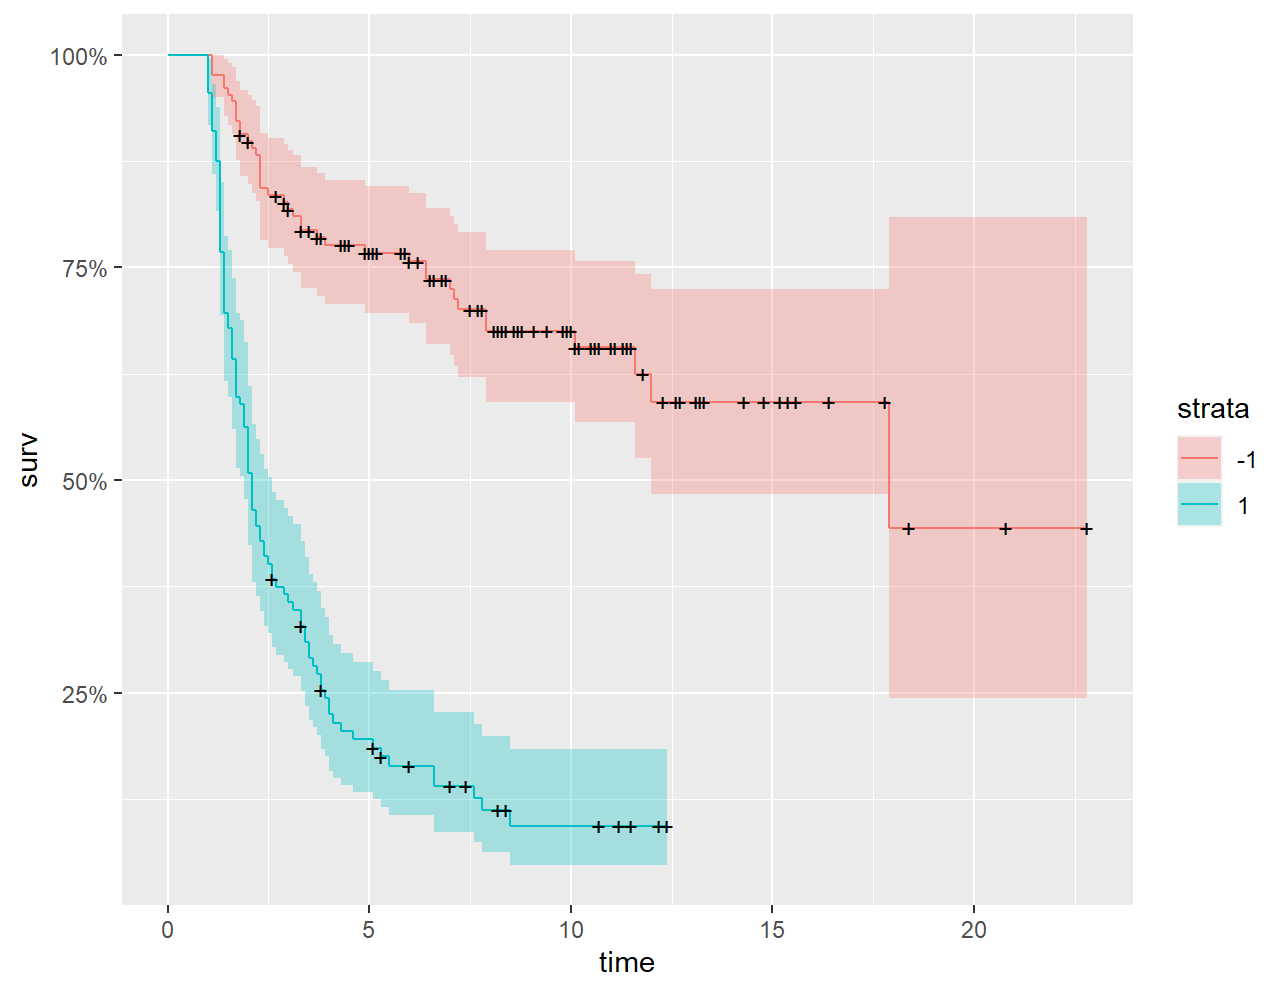
\includegraphics[keepaspectratio, scale=0.7]{kaplanmeiyercurv.png}
\end{figure}

\end{enumerate}
\end{Ex}
%%%%%%%%%%%%%%%%%%%%%%%%%%%%%%%%%%%%32
\begin{Ex}

\end{Ex}
%%%%%%%%%%%%%%%%%%%%%%%%%%33

\section{第3章解答}
\begin{Ex}
\begin{enumerate}[(a)]
  \item $f(x,y)=\sqrt{x^2+y^2}$の$(x,y)\neq (0,0)$における偏微分をそれぞれ求めると
  \begin{align*}
    \frac{\partial f}{\partial x}(x,y)&=\frac{x}{\sqrt{x^2+y^2}}\\
    \frac{\partial f}{\partial y}(x,y)&=\frac{y}{\sqrt{x^2+y^2}}
  \end{align*}
となる.\\

\item $p\geq 2$に対し,$\beta=(\beta_1,\cdots,\beta_p)\neq 0$における$\|\beta\|_2$の$\beta_i(1\leq i\leq p)$における偏微分は
\begin{align*}
  \frac{\partial \|\beta\|}{\partial \beta_i}&=\frac{\beta_i}{\|\beta\|_2}
\end{align*}
となることより,$\|\beta\|_2$の$\beta\neq 0$における偏微分は
$$\frac{\partial \|\beta\|}{\partial \beta}=\frac{\beta}{\|\beta\|_2}$$
となる.\\

\item $f(x,y)$の$(x_0,y_0)=(0,0)$における劣微分を求める.$(u,v)\in\mathbb{R}^2$が劣微分の要素であったとする.すなわち,任意の$(x,y)\in \mathbb{R}^2$に対して
\begin{align}
  \label{retsu}
  f(x,y)\geq ux+vy
\end{align}
を満たしているとする.ここで,$r,s>0,0\leq \theta,\phi< 2\pi$を用いて
\begin{align*}
  x&=r\cos\theta,\quad y =r\sin\theta\\
  u&=s\cos\phi,\quad v = s\sin\phi
\end{align*}
と極座標変換を行うと,(\ref{retsu})式は
\begin{align*}
  r&\geq sr\cos\theta\cos\phi+sr\sin\theta\sin\phi\\
&=rs\cos(\theta-\phi)\\
\therefore 1&\geq s\cos(\theta-\phi)
\end{align*}
とかくことができる.上式が成立することの必要十分条件は$s\geq 1$であることなので,求める劣微分は
$$\{(u,v)\in\mathbb{R}^2\mid u^2+v^2\leq 1\}$$
となる.\qed
\end{enumerate}
\end{Ex}
%%%%%%%%%%%%%%%%%%%%%%%%%%%%%%34

\begin{Ex}
\noindent(a) (3.5)の解が$\beta=0$ $\Leftrightarrow$ $-X^Ty+\lambda\{(u, v)|u^2+v^2\le 1\}\ni (0, 0)$ $\Leftrightarrow$ $||X^Ty||_2\le \lambda$\\[1mm]

\noindent(b)全体の劣微分が0を含むとした式は、


\begin{equation*}
-X^T(y-X\beta +\lambda \frac{\beta}{||\beta||_2})\ni (0, 0)
\end{equation*}

となる。これを変形することで、

\begin{equation*}
X^TX\beta = X^Ty-\lambda \frac{\beta}{||\beta||_2}
\end{equation*}

を得る。
\end{Ex}
%%%%%%%%%%%%%%%%%%%%%%%%%%%%%%%%35
\begin{Ex}

\end{Ex}
%%%%%%%%%%%%%%%%%%%%%%%%%%%%%%%36
\begin{Ex}
$g(z)=\frac{1}{2}(y-Xz)^2$のヘッセ行列$\nabla^2 g(x)$を求めると
\begin{align*}
  \frac{\partial g}{\partial z}(z)&=-X^T(y-Xz)\\
  \frac{\partial g}{\partial z}(z)&=X^TX
\end{align*}
となることがわかる.ここで$X^TX$は非負定値行列であることより,$X^TX$の二次形式の最大値は$X^TX$の最大固有値$\lambda_{max}$に一致するので,任意の$x,y,z\in \mathbb{R}^p$に対して
\begin{align*}
  (x-y)^T \nabla^2g(z)(x-y)&=(x-y)^tX^TX(x-y)\\
  &\leq \lambda_{max}\|x-y\|_2^2
\end{align*}
が成立することがわかる.上式で$\lambda_{max}=L$とすれば求めたい不等式が得られる.\qed\\
\end{Ex}
%%%%%%%%%%%%%%%%%%%%%%%%%%%%%37
\begin{Ex}
\noindent(a)

\noindent(1)$t = 1$のとき、$\alpha_1=1\le 1$より、成立。

\noindent(2)$\alpha_t\ge \frac{t+1}{2}$が成立すると仮定する。このとき、

\begin{equation*}
\alpha_{t+1}=\frac{1+\sqrt{1+4\alpha_t^2}}{2}\ge \frac{1+\sqrt{(t+1)^2}}{2}=\frac{1+(t+1)}{2}=\frac{t+2}{2}
\end{equation*}

より、成立。

\noindent(b)

コードは以下のようになる。

\begin{lstlisting}
def fista(X, y, lam):
    p = X.shape[1]
    nu = 1 / np.max(np.linalg.eigvals(X.T @ X))
    alpha = 1
    beta = np.zeros(p)
    beta_old = np.zeros(p)
    gamma = np.zeros(p)
    eps = 1
    while eps > 0.001:
        w = gamma + nu * X.T @ (y - X @ gamma)
        beta = max(1 - lam * nu / np.linalg.norm(w, 2), 0) * w
        alpha_old = copy.copy(alpha)
        alpha = (1 + np.sqrt(1 + 4 * alpha**2)) / 2
        gamma = beta + (alpha_old - 1) / alpha * (beta - beta_old)
        eps = np.max(np.abs(beta - beta_old))
        beta_old = copy.copy(beta)
    return beta
\end{lstlisting}

実行結果は以下のようになり、問題36と出力が得られた。

\begin{figure}[H]
 \centering
 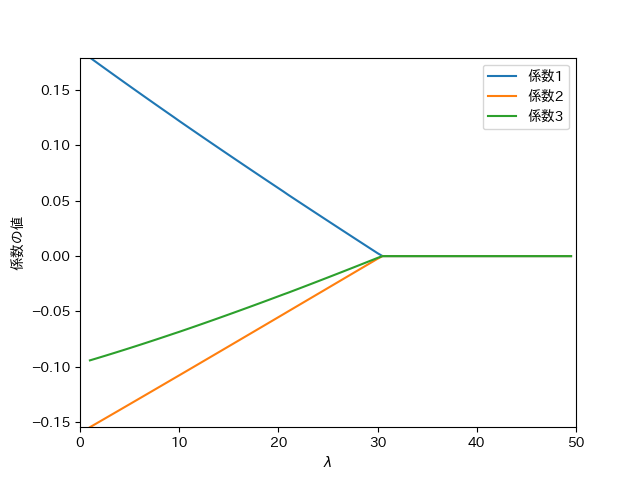
\includegraphics[keepaspectratio, scale=0.7]{fista.png}
\end{figure}
\end{Ex}
%%%%%%%%%%%%%%%%%%%%%%%%%%%%%38
\begin{Ex}

\end{Ex}
%%%%%%%%%%%%%%%%%%%%%%%%%%%%%%%39
\begin{Ex}
  空欄を埋めたプログラムは下の通り.
  \begin{lstlisting}[basicstyle = \ttfamily\footnotesize, frame = single]
def group_lasso(z, y, lam=0):
    J = len(z)
    theta = []
    for i in range(J):
        theta.append(np.zeros(z[i].shape[1]))
    for m in range(10):
        for j in range(J):
            r = copy.copy(y)
            for k in range(J):
                if k != j:
                    r = r - z[k] @ theta[k]
            theta[j] = gr(z[j], r, lam)
    return theta
  \end{lstlisting}

  \begin{lstlisting}[basicstyle = \ttfamily\footnotesize, frame = single]
n = 100
J = 2
u = randn(n)
v = u + randn(n)
s = 0.1 * randn(n)
t = 0.1 * s + randn(n)
y = u + v + s + t + randn(n)
z = []
z = np.array([np.array([u, v]).T, np.array([s, t]).T])
lambda_seq = np.arange(0, 500, 10)
m = len(lambda_seq)
beta = np.zeros((m, 4))
for i in range(m):
    est = group_lasso(z, y, lambda_seq[i])
    beta[i, :] = np.array([est[0][0], est[0][1], est[1][0], est[1][1]])
plt.xlim(0, 500)
plt.ylim(np.min(beta), np.max(beta))
plt.xlabel(r"$\lambda$")
plt.ylabel("係数の値")
labels = ["グループ1", "グループ1", "グループ2", "グループ2"]
cols = ["red", "blue"]
lins = ["solid", "dashed"]
for i in range(4):
    plt.plot(lambda_seq, beta[:, i], color=cols[i//2],
             linestyle=lins[i % 2], label="{}".format(labels[i]))
plt.legend(loc="upper right")
plt.axvline(0, color="black")
plt.show()
    \end{lstlisting}
上記の実行結果は以下の様になる.
\begin{figure}[H]
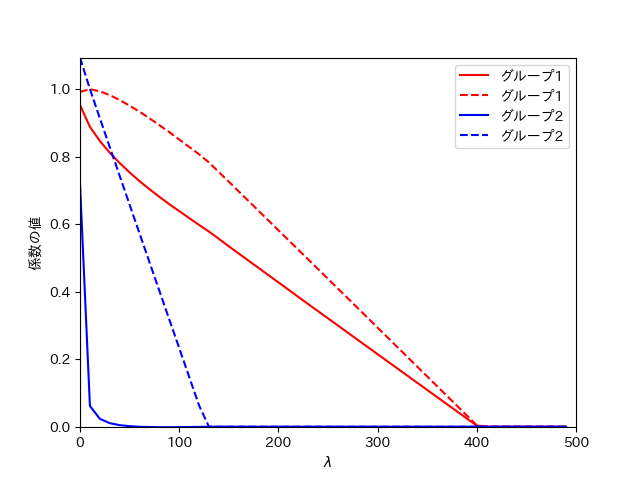
\includegraphics[width=10cm]{gr.png}
\end{figure}
\end{Ex}
%%%%%%%%%%%%%%%%%%%%%%%%%%%%%%%%%%%%%40
\begin{Ex}
\begin{enumerate}[(a)]
\item 関数$\varphi(\theta_k)$を
\begin{align*}
\varphi(\theta_k) =\frac{1}{2}\sum_{i=1}^N(y_i - \sum_{k=1}^Kz_{i,k}\theta_k)^2 + \lambda\sum_{k=1}^K \alpha \|\theta_k\|_1
\end{align*}
と定義する.題意はこの関数の最小値を与える$\theta_k$が$r_{i,k} := y_i - \sum_{l\neq k}z_{i,l}\hat{\theta}_l$として
$$\mathcal{S}_{\lambda \alpha}\left(\sum_{i=1}^N z_{i,k}r_{i,k}\right)$$
でかけることを示すことの誤りであると思われるため,これを考える.\\

まず$\varphi(\theta_k)$を$\theta_k$で劣微分して${\bm 0}$と置いた式は
\begin{align*}
\frac{\partial}{\partial \theta_{k}} \varphi(\theta_k)&=-\sum_{i=1}^N z_{i,k}^T(r_{i,k} - z_{i,k}\theta_k)+\lambda \alpha\begin{cases}
1 & \theta_k > 0\\
[-1,1] &\theta_k = 0\\
-1 & \theta_k < 0
\end{cases}\\
&=\sum_{i=1}^N z_{i,k}^T z_{i,k}\theta_k - \mathcal{S}_{\lambda\alpha}\left(\sum_{i=1}^N  z_{i,k} r_{i,k}\right)\\
& = \theta_k - \mathcal{S}_{\lambda\alpha}\left(\sum_{i=1}^N  z_{i,k} r_{i,k}\right) \ni {\bm 0}
\end{align*}
となる.ただし,$z_{i,k}$が正規化されており$\displaystyle\sum_{i = 1}^N \|z_{i,k}\|_2 ^2 = 1$であることを用いた.$\varphi(\theta_k)$は下に凸な関数であるため,これより$\varphi$の最小値を与える$\theta_lk$が
$$\theta_k = \mathcal{S}_{\lambda\alpha}\left(\sum_{i=1}^N  z_{i,k} r_{i,k}\right)$$
とかけることが示せる.\\

\item (a)の結果より,$\theta_k = 0$が$\varphi(\theta_k)$の最小値となるには各$j(1\leq j\leq p)$に対して
$$-\sum_{i=1}^N r_{i,k}(z_i,k)_j + \lambda \alpha[-1,1] \ni 0\Leftrightarrow -\lambda \alpha \leq \sum_{i=1}^N  (z_{i,k})_j r_{i,k} \leq \lambda \alpha$$
が成立する必要がある.ただし$(z_{i,k})_j$で$z_{i,k}$の第$j$成分を表す.さらに$\varphi(\theta_k)$が$\theta_k = {\bm 0}$で最小であるならば,
\begin{align*}
\frac{1}{2}\sum_{i=1}^N (y_i  - \sum_{k=1}^K z_{i,k}\theta_k)^2 + \lambda\sum_{k=1}^K\{(1-\alpha)\|\theta_k\|_2 + \alpha \|\theta_k\|_1\}
\end{align*}
も$\theta_k = {\bm 0}$で最小になる.以上より上式を$\theta_k$で劣微分して$\theta_k = {\bm 0}$とおけば
\begin{align*}
\mathcal{S}_{\lambda \alpha}\left(\sum_{i=1}^N z_{i,k}r_{i,k}\right ) + \lambda (1-\alpha)s_k& = 0\\
\lambda(1-\alpha)s_k &\ni \mathcal{S}_{\lambda\alpha}\left(\sum_{i=1}^N z_{i,k}r_{i,k}\right)
\end{align*}
が得られる.ただし$s_k$で$\|\theta_k \|$の劣微分を表す.ここで,$\|\theta_k \|$の劣微分は
$$\{\theta_{1,k}^2 + \cdots + \theta_{p_k ,k}^2 < 1\}$$
で書くことができるので,これらより$\theta_k = 0$が解になる必要十分条件が	
\begin{align*}
\lambda(1-\alpha)\{\theta_{1,k}^2 + \cdots +& \theta_{p_k ,k}^2 < 1\}\ni - \mathcal{S}_{\lambda\alpha}\left(\sum_{i=1}^N z_{i,k}r_{i,k}\right)\\
&\Leftrightarrow \lambda(1-\alpha)\leq \left\| \mathcal{S}_{\lambda\alpha}\left(\sum_{i=1}^N z_{i,k}r_{i,k}\right)\right\|_2
\end{align*}
となることがいえる.\\

\item 教科書p.82に沿った議論を行う.通常のグループLassoでは$g(\beta) = \frac{1}{2}\|y - X\beta\|_2^2,h(\beta) = \lambda \|\beta\|_2$,
とした上での勾配法
$$\beta_{t + 1}\leftarrow \beta_t -\nu\{\nabla g(\beta_t) + \partial h(\beta)\}$$
において,近接演算子
$${\rm prox }_h (z) :={\rm argmin}_{\theta \in \mathbb{R}^p}\left\{\frac{1}{2}\|z-\theta\|_2^2 + h(\theta)\right\}$$
による勾配法の書き換え
\begin{align}
\label{groupkoubai}
\beta_{t+1}\leftarrow {\rm prox }_{\nu h}(\beta_t - \nu\nabla g(\beta_t))
\end{align}
の結果として更新式$\beta\leftarrow \left(1-\frac{\nu\lambda}{\|\gamma\|_2}\right)_+ \gamma$が得られた.グループLassoにおいては$g(\beta)$はそのままに,$h(\beta) = \lambda(1-\alpha)\|\beta\|_2 + \lambda \alpha\|\beta\|_1$として同様の議論をしていく.\\

(\ref{groupkoubai})式を具体的に書き下すと
\begin{align*}
{\rm argmin}_{\theta\in\mathbb{R}^p}\left(\frac{1}{2}\|\beta_t - \nu \nabla g(\beta_t) - \theta\|_2^2 + \nu h(\theta)\right)
\end{align*}
となる.被最小化関数を$\theta$で微分すると
\begin{align*}
-(\beta_t - \nu \nabla g(\beta_t) - \theta) + \nu \lambda (1-\alpha)\frac{\theta}{\|\theta\|_2} * \lambda \alpha t_k = 0
\end{align*}
となる.

\end{enumerate}
\end{Ex}
%%%%%%%%%%%%%%%%%%%%%%%%%%%%%%%%%%%%%%41
\begin{Ex}

\end{Ex}
%%%%%%%%%%%%%%%%%%%%%%%%%%%%%%%%%%%%%%42
\begin{Ex}
目的関数$L$は
$$L=\frac{1}{2}\|y-X\sum_{k=1}^K\theta_k\|_2^2 +\lambda\sum_{k=1}^K\|\theta_k\|_2$$
である.ただし
\begin{align*}
  \theta_1=\left(\begin{array}{c}
    \beta_1\\
    \beta_2\\
    \beta_{3,1}\\
    0\\
    0
  \end{array}\right),\quad \theta_2=\left(\begin{array}{c}
    0\\
    0\\
    \beta_{3,2}\\
    \beta_4\\
    \beta_5
  \end{array}\right)\quad (\beta_3=\beta_{3,1}+\beta_{3,2})
\end{align*}
として,$\beta=\theta_1+\theta_2$とした.ここで,$X$の最初の3列を$X_1\in\mathbb{R}^{N\times 3}$,最後の3列を$X_2\in \mathbb{R}^{N\times 3}$と書き,$\theta_1,\theta_2$の非ゼロ成分$\gamma_1,\gamma_2$で$L$に関して劣微分をとると
\begin{align*}
  \frac{\partial L}{\partial \gamma_1}&=-X_1^T(y-X_1\gamma_1)+\lambda\partial\|\gamma_1\|_2\\
  \frac{\partial L}{\partial \gamma_2}&=-X_2^T(y-X_2\gamma_2)+\lambda\partial\|\gamma_2\|_2\\
\end{align*}
と書くことができる.したがって$L$を$\beta$で微分して$0$とおく式は
\begin{align*}
  -X_1^T(y-X\theta_1)+\lambda\partial\|\gamma_1\|_2&=0\\
  -X_2^T(y-X\theta_2)+\lambda\partial\|\gamma_2\|_2&=0
\end{align*}
となるので,上式において$\theta_j=0(j=1,2)$とおくと
\begin{align*}
  X_j^Ty &=\lambda\partial\|\gamma_j\|_2\Leftrightarrow \|X_i^Ty\|_2\leq \lambda\quad(i=1,2)
\end{align*}
となる.最右辺が求める条件である.\qed\\
\end{Ex}
%%%%%%%%%%%%%%%%%%%%%%%%%%%%%%%%%%%%%%%%%%%43
\begin{Ex}
$L_0(\beta)$を$\beta_{j,k}$で偏微分すると、

\begin{equation*}
\sum_{i=1}^{N}\{-x_{i, j}(r^{(j)}_{i,k}-x_{i,j}\beta_{j,k})\}
\end{equation*}

となるので、$L(\beta)$を$\beta_j$で劣微分すると、
\begin{equation*}
\beta_j\sum_{i=1}^{N}x_{i,j}^2-\sum_{i=1}^{N}x_{i,j}r_i^{(j)}+\lambda\partial||\beta_j||_2
\end{equation*}

となる。したがって、

\begin{equation*}
\hat{\beta_j}=\frac{1}{\sum_{i=1}^{N}x_{i,j}^2}(1-\frac{\lambda}{||\sum_{i=1}^{N}x_{i,j}r_i^{(j)}||_2})\sum_{i=1}^{N}x_{i,j}r_i^{(j)}
\end{equation*}

となる。

\end{Ex}
%%%%%%%%%%%%%%%%%%%%%%%%%%%%%%%%%%%%%%%%%%%%%%44
\begin{Ex}

\end{Ex}
%%%%%%%%%%%%%%%%%%%%%%%%%%%%%%%%%%%%%45
\begin{Ex}
  空欄を埋めたプログラムは下の通り
  \begin{lstlisting}[basicstyle = \ttfamily\footnotesize, frame = single]
  def gr_multi_lasso(X, y, lam):
    n = X.shape[0]
    p = X.shape[1]
    K = len(np.unique(y))
    beta = np.ones((p, K))
    Y = np.zeros((n, K))
    for i in range(n):
        Y[i, y[i]] = 1
    eps = 1
    while eps > 0.001:
        gamma = copy.copy(beta)
        eta = X @ beta
        P = np.exp(eta)
        for i in range(n):
            P[i, ] = P[i, ] / np.sum(P[i, ])
        t = 2 * np.max(P*(1-P))
        R = (Y-P) / t
        for j in range(p):
            r = R + X[:, j].reshape(n, 1) @ beta[j, :].reshape(1, K)
            M = X[:, j] @ r
            beta[j, :] = (max(1 - lam / t / np.sqrt(np.sum(M*M)), 0)
                          / np.sum(X[:, j]*X[:, j]) * M)
            R = r - X[:, j].reshape(n, 1) @ beta[j, :].reshape(1, K)
        eps = np.linalg.norm(beta - gamma)
    return beta
\end{lstlisting}


\begin{lstlisting}[basicstyle = \ttfamily\footnotesize, frame = single]
  iris = load_iris()
  X = np.array(iris["data"])
  y = np.array(iris["target"])
  
  lambda_seq = np.arange(10, 151, 10)
  m = len(lambda_seq)
  p = X.shape[1]
  K = 3
  alpha = np.zeros((m, p, K))
  for i in range(m):
      res = gr_multi_lasso(X, y, lambda_seq[i])
      alpha[i, :, :] = res
  plt.xlim(0, 150)
  plt.ylim(np.min(alpha), np.max(alpha))
  plt.xlabel(r"$\lambda$")
  plt.ylabel("係数の値")
  handles = []
  labels = ["がく片の長さ", "がく片の幅", "花びらの長さ", "花びらの幅"]
  cols = ["red", "green", "blue", "cyan"]
  for i in range(4):
      for k in range(K):
          line, = plt.plot(lambda_seq, alpha[:, i, k], color=cols[i],
                           label="{}".format(labels[i]))
      handles.append(line)
  plt.legend(handles, labels, loc="upper right")
\end{lstlisting}
また実行結果は下の通り
\begin{figure}[H]
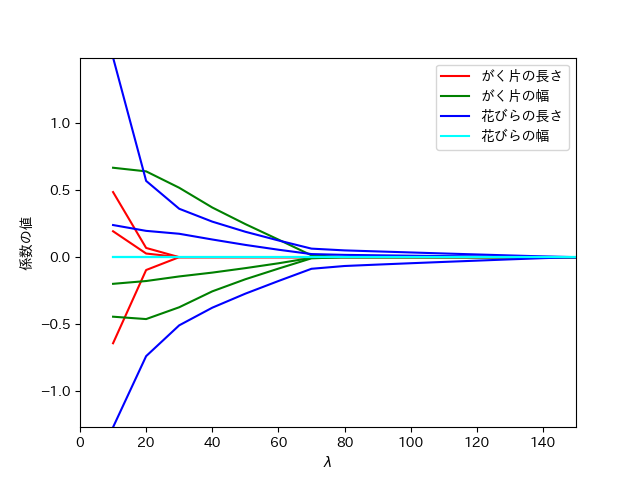
\includegraphics[width=10cm]{iris.png}
 \end{figure}
\end{Ex}
%%%%%%%%%%%%%%%%%%%%%%%%%%%%%%%%%%%%46
\end{document}